\documentclass[a4paper,kul]{kulakarticle} 

\usepackage[utf8]{inputenc}
\usepackage[dutch]{babel}

\address{
	Project ontwerpen in ... \\
	promotor\\
	assistenten}
\date{Academiejaar 2020-2021}
\title{Opdrachtsverklaring}
\author{Bas C, Sofie m, Nele Eeckman}

\begin{document}
	\maketitle
	
%	\section*{Inhoud project}
%	- een bijgestelde formulering van de ontwerpopdracht, met numerieke ontwerpspecificaties waar van toepassing
%	
%	- een tijdsplanning, bv. aan de hand van een Gantt-chart
%	
%	To help you further with your plan, ask yourselves the following question:
%	*Do you already have the required knowledge to complete the tasks you mentioned yourselves?
%	*If no, how would you acquire this knowledge? (literature?)
%	*How to integrate the algorithms in the framework?
%	*What about testing the integration?
%	*What about intermediate and final tests of the complete framework?
%	*What are the specifics of the GUI/
%	*Is it possible to gradually build up the GUI? What are the essential components?
%	*Think about the complete framework. Say that you have the complete setup (mobile EEG + a laptop + ...) and you press 'Start', what happens? What chain of actions occurs? 
%	
%	Try to think about the whole framework and each individual component. Note that the tasks you have already outlined are already a good start.
	
		\section*{Inhoud project}
	
	\subsection*{Achtergrond}
	Mensen met gehoorproblemen hebben veel moeite met het onderscheiden van spraakbronnen in rumoerige omgevingen. De meeste hoortoestellen zijn daarom uitgerust met een algoritme dat achtergrondgeluid tracht te onderdrukken. In zogenaamde `\textit{cocktail party}'-scenario's met meerdere sprekers moet dat soort algoritme echter weten naar welke spreker de gebruiker wil luisteren en wie of wat als achtergrondlawaai moet worden behandeld. In plaats van suboptimale heuristische regels te gebruiken, bijvoorbeeld op basis van de kijkrichting, zijn nieuwe algoritmen gepubliceerd op basis van auditieve aandacht decodering (AAD). Deze algoritmen maken het mogelijk de bijgewoonde spreker te decoderen op basis van de hersensignalen die worden verzameld door elektro-encefalografie (EEG)-sensoren.
	
	\subsection*{Omschrijving}
	Het project moet resulteren in een volledig operationeel \textit{proof of concept} van een \textit{real-time} EEG-gebaseerd AAD-systeem dat zowel voor onderzoek als voor demonstratiedoeleinden kan worden gebruikt. Dit houdt in dat de auditieve aandacht met behulp van een 24-kanaal, draagbaar EEG-systeem in \textit{realtime} wordt bepaald wanneer twee concurrerende luidsprekers gelijktijdig aan het onderwerp worden gepresenteerd. Aan de hand van de informatie die gehaald wordt uit EEG-signalen zal het volume van de spreker en de omgeving geregeld worden. Het is belangrijk dat er gewerkt wordt met een \textit{closed loop} systeem zodat \textit{feedback} mogelijk wordt in het geval van een verkeerde keuze. In zo'n systeem wordt de verkozen spreker duidelijk gemaakt aan de gebruiker. Indien de gebruiker daarentegen naar de andere spreker wilt luisteren kan deze hier onmiddelijk op reageren door zich op die andere spreker te focusen. \\
	Het AAD algoritme moet zowel een functionaliteit op basis van stimulusreconstructie als directionele focus bevatten. Dit eerste vereist synchronisatie tussen de spraakstimulus en de EEG-signalen. Hierbij wordt de spraakinput gesplitst in de individuele spraaksignalen van de verschillende sprekers. Vanuit de hersensignalen die worden ingelezen met behulp van EEG wordt het beluisterde spraaksignaal gerecreëerd. Die wordt dan vergeleken met de opgesplitste spraakinput om te bepalen naar wie er wordt geluisterd.\\
	De directionele focus functionaliteit deelt twee spraakstimuli in in een categorie voor links of een voor rechts. Met behulp van de EEG wordt dan de richting van het beluisterde signaal bepaald.\\ %hier aanvulling nodig?
	Er zal een GUI (\textit{graphical user interface}) met Python gebouwd worden, die de decoderingsresultaten zal visualiseren, zodat de \textit{realtime neurofeedback} mogelijk is.\\
	Voor dit project wordt een laptop en een draagbare EEG voorzien. Als eerste moet een AAD algoritme worden opgesteld. In een EEG-meetnamiddag zal data verworven worden. Hiermee kan het algoritme getraind worden zodat het \textit{realtime} beslissingen zou kunnen nemen. De tijdslimiet voor het nemen van deze beslissingen wordt op tien seconden gesteld. Indien mogelijk kan deze limiet verder geminimaliseerd worden zolang er geen een beduidende daling in nauwkeurigheid optreedt. Dit \textit{realtime} algoritme kan dan geïmplementeerd worden in een \textit{realtime} framework. Het framework bestaat al, maar moet nog geoptimaliseerd worden.\\
	Hieronder worden de belangrijkste specificaties nog eens opgelijst:
	\begin{itemize}
		\item Materiaal: laptop, draagbare EEG (24-kanaal)
		\item Gebruiksvriendelijke GUI
		\item Simpele opbouw, zodat het eenvoudig uitgebreid kan worden als er een nieuwe aanpak mogelijk blijkt te zijn.
		\item \textit{Closed loop}
		\item Korte beslissingstijd, zonder relevante verliezen in nauwkeurigheid
	\end{itemize}
	

	\section*{Planning}
	De opbouw van het project kan opgedeeld worden in vier onderdelen: de project inleiding, het software ontwerp, de experimenten en de rapportering. De projectplanning wordt weergegeven in Figuur \ref{fig:ganttchart}.
	
	\subsection*{Project inleiding}
	Deze eerste weken van het project bestaan uit een korte inleiding om beter vertrouwd te raken met de inhoud van het project. Om beter begrip van \textit{neuro steered hearing devices} en AAD te verkrijgen wordt er eerst een verkennende literatuurstudie uitgevoerd. Na het lezen van enkele papers rond dit onderwerp volgt er research naar welke toepassingen op dit moment al ter beschikking zijn in Python.\\
	
	
	\subsection*{Software ontwerp}
	In het onderdeel ontwerpen wordt de nodige \textit{software} volledig op punt gesteld. Het algoritme bestaat uit drie belangrijke bouwblokken. Als eerste zal het algoritme voor AAD met directionele focus opgesteld worden. Daarna wordt dit algoritme uitgebreid met de AAD door middel van stimulus reconstructie. Als laatste wordt een gebruiksvriendelijke GUI opgesteld. Voor elk onderdeel wordt er tijd voorzien voor de implementatie en voor de integratie in het voorziene framework.\\
	
	\subsection*{Experimenten}
	In het onderdeel Experimenten wordt een meetnamiddag gepland met als doel het efficient gebruiken van een EEG beter te begrijpen en data te verwerven. Daarnaast zal de \textit{software} eens die klaar is, in praktijk getest moeten worden. Hierbij moet er zeker gecontroleerd worden of de GUI gebruiksvriendelijk is en de \textit{closed loop} correct gebruikt kan worden.\\
	
	\subsection*{Rapportering}
	De rapportering bestaat uit een eind verslag, tussentijdse presentatie en eind presentatie. Hiervoor wordt telkens de nodige voorbereidingstijd voorzien. De tussentijdse presentatie vindt plaats in de laatste lesweek in december. Daarna moet op 10 mei het definitieve verslag worden ingediend. De eind presentatie zal plaatsvinden tijdens de laatste lesweek in mei.\\
	
		
\begin{figure}[h]
		%\centering
		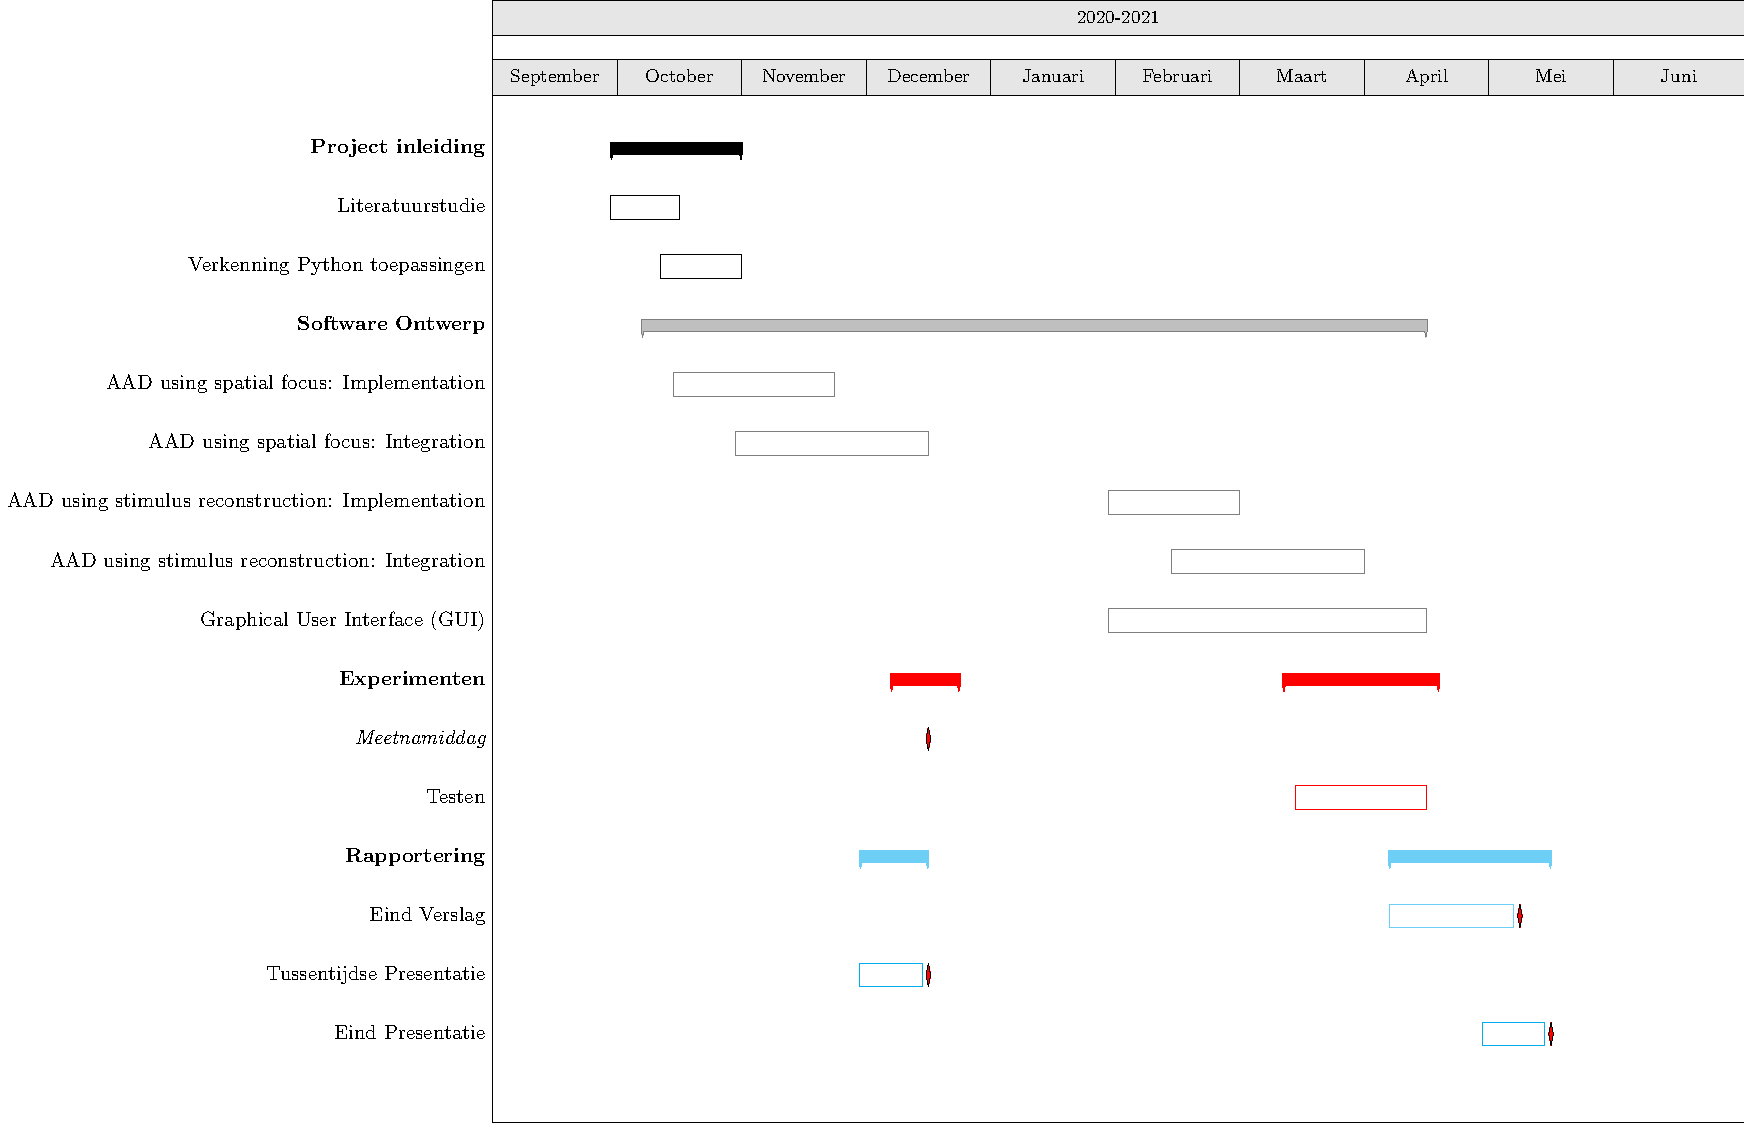
\includegraphics[scale=0.55]{Ganttchart2.pdf} 
		\caption{Projectplanning voorgesteld aan de hand van een Gantt-chart.}
		\label{fig:ganttchart}
	\end{figure}
	
\end{document}	
	
\end{document}	
	